

% Niveau :      PCSI *
% Discipline :  Méca
% Mots clés :   Trajectoire particule chargée

\begin{exercise}{Minimum de déviation}{1}{Spé}
{Optique ondulatoire, Réseau}{bermu}

On considère une onde plane progressive harmonique, de longueur d'onde $\lambda$ en incidence $\theta$ sur un réseau de diffraction plan en transmission de pas $a = \SI{100}{µm}$.

\begin{questions}
\questioncours Donner la relation fondamentale des réseaux.

\uplevel{On appelle déviation l'angle $D$ entre les directions incidente et diffractée.}

\question Calculer le minimum de déviation du réseau.

\end{questions}
\end{exercise} 

\begin{solution}


\begin{questions}
\questioncours $\sin\theta' - \sin\theta = p\lambda/a$

\question $D = \theta' - \theta$. Le minimum est donc pour $\dv{\theta' - \theta}{\theta} = 0$ donc $\dv{\theta'}{\theta} = 1$.

Or $\sin\theta' - \sin\theta = p\lambda/a$, donc par dérivation $\cos\theta' = \cos\theta$. Donc plusieurs cas

\begin{itemize}
    \item $\theta = \theta'$ : $D_m = 2\theta$ (réseaux en transmission)
    \item $\theta = -\theta'$ : $D_m = 0$ (réseaux en réflexion)
\end{itemize}
\end{questions}

\end{solution}



\begin{exercise}{Réseau blazé}{2}{Spé}
{Optique ondulatoire, Réseau}{bermu}

On considère un réseau de diffraction plan en réflexion de pas $a$ éclairé en incidence $i$ par un faisceau parallèle de lumière monochromatique de longueur d'onde $\lambda = 530$ nm.

\begin{questions}

\questioncours Donner la formule des réseaux.

\question Quelle est la différence de marche entre deux rayons frappant deux motifs successifs sous la même incidence $i$ et émergeant sous l’angle $i’$ ? \`A quelle condition observe-t-on un maximum de l’éclairement du aux interférences ? Comment évolue l'intensité de ces maxima en fonction de l'ordre ?

\uplevel{Un réseau blazé est obtenu en traçant sur une surface métallique des dents de scie dont la coupe
est représentée ci-contre. Les bandes utiles réfléchissantes ont pour largeur $b$, sont inclinées d'un angle $\alpha$ et constituent un réseau de $N$ bandes de pas $a$.
\begin{figure}[H]
    \centering
    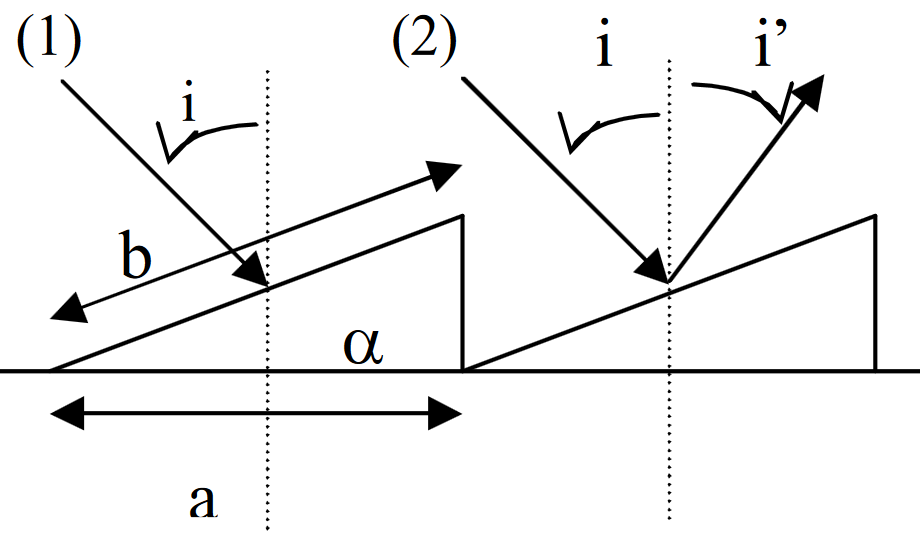
\includegraphics[width=0.4\linewidth]{optique/interferences/reseau-blaze.png}
    \caption{Schéma de principe d'un réseau blasé.}
\end{figure}

On observe les ondes diffractées dans la direction $i'$ à l'infini.
}

\question D'après ce que vous savez sur l'optique géométrique, en quel angle $i_0'$ se trouvera le maximum de diffraction ?

\question On souhaite faire coïncider ce maximum de diffraction avec le maximum d'interférence de l'ordre $p$. Quelle relation doit alors vérifier l'angle de blaze $\alpha_p$ ? En quoi cela est intéressant contrairement à un réseau plan simple ?

\question Le réseau utilisé comporte 200 motifs/mm. Il est utilisé en autocollimation ($i=0$) et concentre l’énergie
dans l’ordre 4. Donner l'angle de blaze de ce réseau. Comment pourriez-vous distinguer expérimentalement ce réseau d’un réseau plan ?

\end{questions}
\end{exercise} 

\begin{solution}


\begin{questions}
\questioncours $\sin i' - \sin i = p\lambda/a$

\question $\delta = a(\sin i' - \sin i) = -p\lambda$.

L'intensité des maxima diminue dramatiquement avec l'ordre. Presque tout est concentré dans l'ordre 0, ce qui est bête.

\question L'angle max est l'angle de réflexion des lois de Descartes. $\theta = \theta'$ (par rapport à la normale au dioptre) soit $i - \alpha = i' + \alpha$. $i = i' + 2\alpha$.

\question Pour coïncider avec $i'_p$ tel que $a(\sin i'_p - \sin i) = -p\lambda$, avec également $i'_p = i - 2\alpha$, on veut $$\sin (2\alpha - i) + \sin i = p\lambda/a.$$

La lumière est maintenant dans l'ordre $p$ ce qui est quand même plus intéressant.

\question On veut donc $\sin (2\alpha) = 4\lambda/a$ (...)

On le distingue par le fait que l'ordre 0 est peu lumineux i.e. on ne voit ce qu'il y a en face pas au travers.
\end{questions}

\end{solution}





% Niveau :      PCSI *
% Discipline :  Méca
% Mots clés :   Trajectoire particule chargée

\begin{exercise}{Pouvoir de résolution du réseau}{3}{Spé}
{Optique ondulatoire, Réseau}{bermu}

On considère une onde plane progressive harmonique, de longueur d'onde $\lambda$ en incidence normale sur un réseau de diffraction plan en transmission de pas $a = \SI{100}{µm}$.

\begin{questions}
\questioncours Décrire le principe du réseau.

\question Établir la différence de marche entre deux ondes issues de deux fentes consécutives du réseau dans la direction $\theta$. Pour quelles directions aura-t-on des interférences constructives ?

\question Calculer amplitude complexe de l'onde lumineuse à l'infini dans la direction $\theta$. On notera $N$ le nombre de fentes (uniformément) éclairées par l'onde incidente.

\question Calculer l'intensité lumineuse de l'onde à l'infini $I(\theta)$. Quelles sont les maxima de l'intensité ? Donner la largeur angulaire $\delta\theta$ des pics d'intensité maximale.

\uplevel{On considère maintenant le réseau éclairé en lumière polychromatique. On appelle pouvoir de résolution la quantité $P = \dfrac{\lambda_m}{\delta\lambda_m}$, ou $\delta \lambda_m$ est la différence minimale entre deux longueurs d'onde que le système peut séparer, et $\lambda_m$ leur moyenne.}

\question Rappeler le critère de Rayleigh sur la résolution de deux pics $\theta_1$ et $\theta_2$ dont la largeur angulaire est $\delta\theta$.

\question \`A l'aide des questions précédentes, établir le pouvoir de résolution de ce réseau.

\end{questions}
\end{exercise} 

\begin{solution}

\begin{questions}
\questioncours Des trous de taille $a$...

\question Faire un beau schéma. $\delta = a\sin\theta$. On a donc interférence pour $p = \delta/\lambda$ entier soit
$$\sin\theta_p = p\lambda/a.$$

\question $s(\theta) = \sum_{k=0}^{N} s_0 e^{i2\pi k \delta/\lambda} = s_0 \dfrac{e^{i2\pi N \delta/\lambda} - 1}{e^{i2\pi \delta/\lambda} - 1} = s_0 e^{i2\pi (N-1) \delta / \lambda} \dfrac{\sin(\frac{N\pi\delta}{\lambda})}{\sin(\frac{\pi\delta}{\lambda})}.$

\question $I(\theta) = I_0 \dfrac{\sin^2\qty(\frac{N\pi\delta}{\lambda})}{\sin^2\qty(\frac{\pi\delta}{\lambda})}.$
Maximum en $\theta = \theta_p$. Autour $\theta = \theta_p \pm \delta\theta/2$, on annule le numérateur si $N\pi\delta/\lambda = (p\pm1)\pi$, soit $\sin(\theta_p \pm \delta\theta/2) = \frac{p\pm1}{a N}$ soit
$$\delta\theta = \dfrac{2\lambda}{N a \cos\theta_p}$$

\question Critère de Rayleigh : $\theta_1 - \theta_2 > \delta\theta/2$.

\question Ainsi, on doit avoir : $\theta(\lambda_m + \delta\lambda/2) - \theta(\lambda_m - \delta\lambda/2) > \dfrac{2\lambda}{N a \cos\theta_p}$ et comme $\sin\theta_p = p\lambda/a$ :
$$\sin\theta(\lambda_m + \delta\lambda/2) - \sin\theta(\lambda_m - \delta\lambda/2) = 2 p\delta\lambda/a \cos\theta_p$$
enfin
$$\delta\lambda = \lambda/ pN \qqtext{soit} P = pN.$$


\end{questions}

\end{solution}
